\section{系统组成及功能说明}

\subsection{整体介绍}

系统由 AI PC、KV260 和机械臂组成，分工见图~\ref{fig:arch}。AI PC 的 NPU 处理头部相机图像，GPU 运行本地大模型，CPU 进行坐标变换、逆运动学求解与轨迹检查。KV260 的 ARM 处理器（PS）管理作业并运行腕部定位，PL 按 5\ms 周期求值轨迹、调度 CAN 发送，同时执行保护和受限修正。六轴机械臂与夹爪共七个电机接收设定，完成抓取和放置。\doccite{ref:kv260}

头部相机覆盖两个托盘，提供接近目标所需的全局位置；腕部相机在抓取前测量局部偏差。作业包经千兆网线下发到 KV260，连续对准在板内完成。放置结束后，头部相机再次观察目标盘，核对实际结果是否满足任务要求。

\begin{figure}[H]
\centering
\resizebox{\linewidth}{!}{%
\begin{tikzpicture}[
  font=\footnotesize,
  blk/.style={draw=#1!60!black,fill=#1!7,rounded corners=2pt,align=center,minimum height=9mm,text width=27mm},
  blk/.default=blue,
  wide/.style={draw=#1!60!black,fill=#1!7,rounded corners=2pt,align=center,minimum height=9mm,text width=61mm},
  grp/.style={draw=#1!70!black,rounded corners=4pt,inner sep=3mm,thick},
  ar/.style={-{Stealth[length=1.8mm]},semithick},
  lab/.style={font=\scriptsize,inner sep=1.5pt}]
  % AI PC: two input columns feeding one planner
  \node[blk=teal] (cmd) at (0,0) {中文指令};
  \node[blk=teal] (cam) at (34mm,0) {头部相机 D435i\\USB3};
  \node[blk=teal] (llm) at (0,-15mm) {指令理解\\Qwen2.5-VL · \textbf{GPU}};
  \node[blk=teal] (det) at (34mm,-15mm) {零件分割 YOLO11n-seg\\\textbf{NPU} · A8W8};
  \node[wide=teal] (plan) at (17mm,-31mm) {CPU 规划与轨迹检查\\逆运动学 · 轨迹 · MuJoCo};
  \node[wide=teal] (ui) at (17mm,-46mm) {上位机控制台\\核对 · 中文复审 · 示教 · 数字孪生};
  % KV260
  \node[blk=orange] (exe) at (88mm,-31mm) {PS 作业执行\\校验 · 执行链 · 心跳};
  \node[blk=orange] (vl) at (122mm,-31mm) {PS 腕部视觉环\\定位 · 误差 · 修正};
  \node[draw=red!60!black,fill=red!6,rounded corners=2pt,align=center,minimum height=12mm,text width=62mm] (pl) at (105mm,-53mm) {\textbf{PL（100 MHz）}\\5 ms 轨迹求值 · CAN 调度 · 守护 · 看门狗\\图像掩码核 · 在线修正通道};
  % devices
  \node[blk=gray] (wc) at (122mm,-8mm) {腕部相机 OV9281};
  \node[blk=gray,text width=44mm] (arm) at (105mm,-77mm) {EDULite A3 六轴 + 夹爪 · 7 电机};
  \begin{scope}[on background layer]
    \node[grp=teal,fit=(cmd)(cam)(ui),label={[font=\small\bfseries]above:Ryzen AI PC}] {};
    \node[grp=orange,fit=(exe)(vl)(pl),label={[font=\small\bfseries,anchor=south west]north west:Kria KV260}] {};
  \end{scope}
  \draw[ar] (cmd)--(llm); \draw[ar] (cam)--(det);
  \draw[ar] (llm.south)--(llm.south|-plan.north); \draw[ar] (det.south)--(det.south|-plan.north);
  \draw[ar] (plan)--(ui);
  \draw[ar] (plan.east)--node[lab,above,pos=.4]{作业包}node[lab,below,pos=.4]{千兆直连}(exe.west);
  \draw[ar] (wc)--node[lab,right,pos=.25]{USB}(vl);
  \draw[ar] (exe.south)--node[lab,left]{AXI-Lite}(exe.south|-pl.north);
  \draw[ar] (vl.south)--node[lab,right]{修正目标}(vl.south|-pl.north);
  \draw[ar,<->] (pl)--node[lab,right,pos=.72]{CAN 1 Mbps}(arm);
\end{tikzpicture}
}
\caption{系统整体框图}\label{fig:arch}
\end{figure}

一次分拣任务的数据流如下：

\begin{enumerate}
  \item \textbf{理解}：操作员输入中文指令，规则解析或本地大模型生成任务合约（零件类别、数量、目标托盘）。
  \item \textbf{感知}：NPU 对头部相机画面做实例分割，结合深度换算出每个零件在机械臂基座坐标系中的位置与主轴方向。
  \item \textbf{规划}：逆运动学与七次多项式生成关节轨迹，MuJoCo 模型逐段检查碰撞与几何约束，打包成作业包下发。\doccite{ref:trajectory}
  \item \textbf{执行}：KV260 校验作业后把多项式段原子提交给 PL，PL 每 5\ms 求值并经 CAN 发送位置设定。
  \item \textbf{对准}：到达零件上方后，腕部视觉环把像素误差换算为关节偏移写入 PL 修正通道，收敛后下降夹取。
  \item \textbf{核验}：放置完成后回到起点，头部相机逐槽核对，本地大模型对比前后画面给出中文复审。
\end{enumerate}

模型推理与规划放在 AI PC，局部视觉定位放在板端 ARM，定时执行与设定检查放在 PL，具体划分见表~\ref{tab:partition}。

\begin{table}[H]
\centering\small
\caption{软硬件划分依据}\label{tab:partition}
\begin{tabularx}{\linewidth}{@{}>{\raggedright\arraybackslash}p{4.1cm} >{\raggedright\arraybackslash}p{2.2cm} Y@{}}
\toprule
功能 & 位置 & 依据 \\
\midrule
检测、语言理解、规划、校验 & AI PC & 计算量大、算法迭代快；NPU/GPU 本地推理，CPU 规划 \\
轨迹插补与 5\ms 设定发送 & PL & 节拍由 PL 计数器与截止期队列保证，不受 Linux 调度影响 \\
租约、反馈新鲜度、编码范围守护 & PL & 与发送路径同一时钟域，按故障类型限制后续发送 \\
七轴跟踪看门狗 & PL & 逐反馈帧判定七轴，不增加总线负载 \\
腕部图像掩码 & PL & 大螺丝路径的掩码处理 P50 7.82\ms，减少 CPU 耗时 \\
在线修正 & PS 与 PL & PS 只写目标，PL 逐拍限幅限速，对准环不经网络 \\
\bottomrule
\end{tabularx}
\end{table}

\subsection{硬件系统介绍}

\subsubsection{硬件整体介绍}

\begin{table}[H]
\centering\small
\caption{硬件组成}\label{tab:bom}
\begin{tabularx}{\linewidth}{@{}>{\raggedright\arraybackslash}p{1.8cm} >{\raggedright\arraybackslash}p{4.6cm} Y@{}}
\toprule
类别 & 器件 & 主要功能与连接 \\
\midrule
计算主机 & AMD Ryzen AI 9 HX PRO 370 & XDNA2 NPU 分割零件；Radeon 890M 运行大模型；CPU 规划轨迹 \\
控制板 & Kria KV260（K26 SOM） & ARM 管理作业与视觉定位；PL 定时控制、执行保护及掩码加速 \\
执行机构 & EDULite A3 六轴机械臂与夹爪 & 六个关节电机定位末端，夹爪电机完成开合；CAN 1\,Mbps \\
总线接口 & SN65HVD230（3.3\,V） & 连接 PL 逻辑电平与 CAN 差分总线；两端 120\,$\Omega$ 终端 \\
头部相机 & Intel RealSense D435i & USB3 接 AI PC，采集彩色图像与深度，覆盖两个托盘 \\
腕部相机 & OV9281 全局快门 USB 相机 & 固定于夹爪本体，直连 KV260，输出 640×400 灰度图供局部对准 \\
工作台 & 左右两个托盘 & 右盘记为 A，左盘记为 B；B 盘配置 5 个放置槽位 \\

\bottomrule
\end{tabularx}
\end{table}

KV260 与 CAN 收发器经 PMOD J2 连接：J2-1 为 \texttt{can\_tx}（H12，LVCMOS33），J2-3 为 \texttt{can\_rx}（E10），J2-9 为地，J2-11 为 3.3\,V 供电。机械臂独立供电，与 KV260 通过 CAN 差分线和信号地相连。\doccite{ref:can}\doccite{ref:transceiver}

\subsubsection{机械设计介绍}

工位由机械臂、两个托盘和相机支架组成。头部 D435i 固定在托盘上方，同时覆盖两个托盘；腕部相机固定在夹爪的不动本体上，开合时支架不随爪指移动，镜头对焦于抓取对准距离。机械臂 URDF 模型用于正运动学计算、MuJoCo 轨迹检查及数字孪生显示，头部相机及立柱作为静态障碍物参与规划。\doccite{ref:realsense}\doccite{ref:mujoco}\doccite{ref:robotics}

\begin{figure}[H]
  \centering
  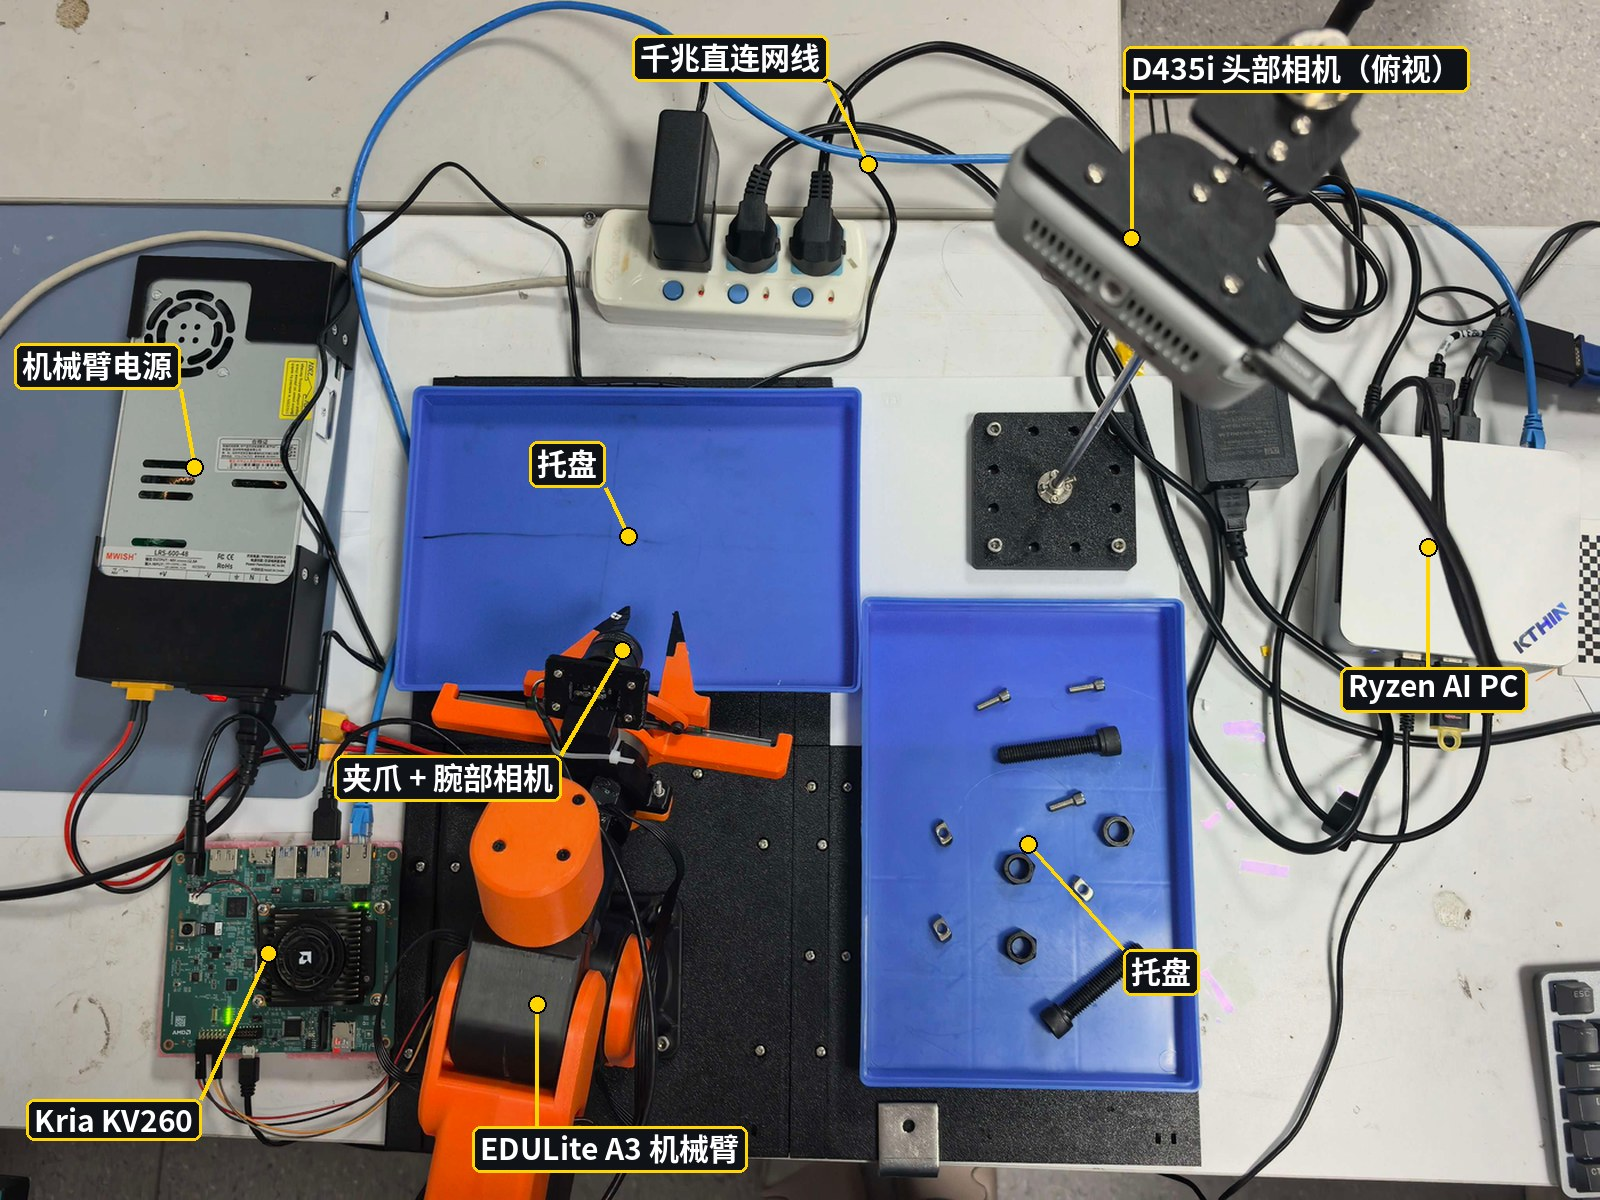
\includegraphics[width=.9\linewidth]{workcell_layout.jpg}
  \caption{工位布局（俯视）}\label{fig:mech}
\end{figure}

\begin{figure}[H]
  \centering
  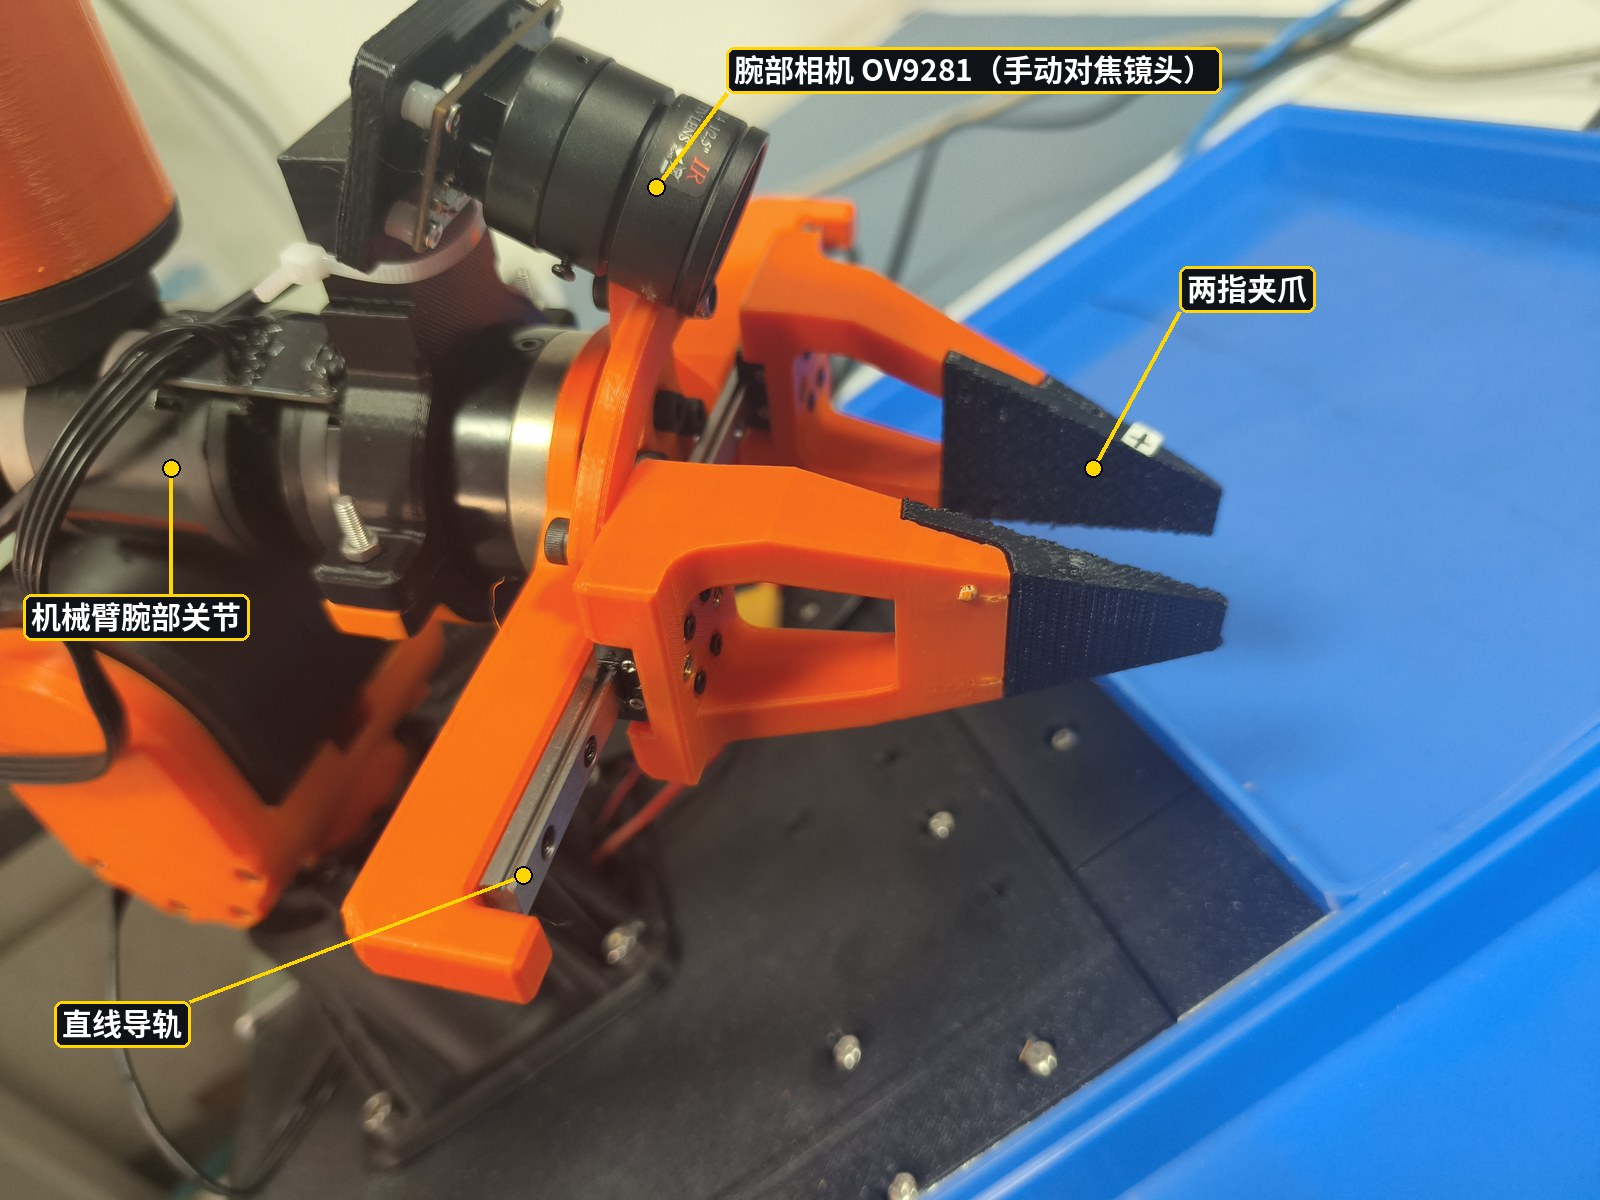
\includegraphics[width=.62\linewidth]{gripper_wrist_camera.jpg}
  \caption{两指夹爪与腕部相机}\label{fig:gripper}
\end{figure}

\subsubsection{电路各模块介绍（KV260 PL 设计）}

PL 内的控制与加速模块运行在 100\,MHz 时钟域，经 AXI-Lite（UIO 窗口）与 PS 交互，视觉核另有 \texttt{m\_axi} 主口直接读帧写掩码（图~\ref{fig:pl}，表~\ref{tab:pl}）。

\begin{figure}[H]
\centering
\resizebox{\linewidth}{!}{%
\begin{tikzpicture}[
  font=\footnotesize,
  m/.style={draw=red!60!black,fill=red!6,rounded corners=2pt,align=center,minimum height=10mm,text width=33mm},
  ps/.style={draw=orange!60!black,fill=orange!8,rounded corners=2pt,align=center,minimum height=10mm,text width=22mm},
  ex/.style={draw=gray!70,fill=gray!10,rounded corners=2pt,align=center,minimum height=10mm,text width=22mm},
  ar/.style={-{Stealth[length=1.6mm]},semithick},
  lab/.style={font=\scriptsize,inner sep=1.5pt}]
  \node[ps] (a53) at (-3mm,0) {PS · A53\\作业执行 · 视觉环};
  \node[ps] (ddr) at (-3mm,-36mm) {DDR\\腕部帧 · 掩码};
  \node[m] (ts) at (44mm,0) {\textsf{trajectory\_stream}\\HLS 七次多项式求值\\在线修正通道};
  \node[m] (ce) at (44mm,-18mm) {\textsf{can\_engine}\\调度 · 租约 · 新鲜度守护};
  \node[m] (vp) at (44mm,-36mm) {HLS \textsf{vision\_pre}\\填充 · 高斯 · Otsu · 闭运算};
  \node[m,text width=24mm] (cc) at (82mm,-18mm) {CAN 位级控制器};
  \node[m,text width=24mm] (tm) at (82mm,0) {\textsf{tracking\_}\allowbreak\textsf{monitor}\\七轴看门狗};
  \node[ex] (tr) at (118mm,-18mm) {SN65HVD230\\7 个电机};
  \begin{scope}[on background layer]
    \node[draw=red!70!black,thick,rounded corners=4pt,fit=(ts)(vp)(cc)(tm),inner sep=3mm,label={[font=\small\bfseries]above:PL（100 MHz 单时钟域）}] {};
  \end{scope}
  \draw[ar,<->] (a53)--node[lab,above]{AXI-Lite}node[lab,below]{UIO 寄存器}(ts);
  \draw[ar] (ts)--node[lab,right]{每 5 ms 设定}(ce);
  \draw[ar] (ce)--(cc);
  \draw[ar,<->] (cc)--node[lab,above]{CAN}node[lab,below]{1 Mbps}(tr);
  \draw[ar] (cc)--node[lab,right]{旁听收发帧}(tm);
  \draw[ar,<->] (ddr)--node[lab,above]{m\_axi}node[lab,below]{DMA}(vp);
  \draw[ar] (a53)--node[lab,left]{写入帧}(ddr);
\end{tikzpicture}
}
\caption{KV260 PL 模块结构}\label{fig:pl}
\end{figure}

\begin{table}[H]
\centering\small
\caption{PL 模块功能与实测}\label{tab:pl}
\begin{tabularx}{\linewidth}{@{}>{\raggedright\arraybackslash}p{3.3cm} Y Y@{}}
\toprule
模块 & 功能 & 实测 \\
\midrule
\path{trajectory_stream} + HLS \texttt{trajectory\_eval} & 每 5\ms 求值七次多项式（Q8.24），生成 Type18 位置设定；截止期队列；原子提交多项式段 & 线上周期偏差 P50 0.4\us；控制服务暂停时最长命令间隔 PL 5.014\ms，ARM 21.435\ms \\
在线修正通道 & 六关节偏移在求值后叠加；每关节限幅、每拍限速、租约；越界故障 & 179 拍逐拍检查与 16/16 回归通过 \\
\texttt{can\_engine} & CAN 收发、反馈表、租约 100\ms、反馈新鲜度、编码范围守护 & 1\,Mbps，总线占用 26.8\% \\
\path{tracking_monitor} & 被动旁听设定帧与反馈帧，七轴跟踪误差看门狗 & 检测延迟 PL 300.8\ms，ARM 判据 408.1\ms \\
HLS \texttt{vision\_pre} & 手指区填充、11 抽头高斯、ROI 内 Otsu、阈值、7×7 闭运算，DMA 读帧写掩码 & 7.82\ms（ARM 14.43\ms），每帧 CPU 0.68\ms；与 ARM 参考逐位一致 \\
\bottomrule
\end{tabularx}
\end{table}

CAN 位级收发采用开源 freecores CAN 控制器（LGPL，保留版权与修改记录）\doccite{ref:freecores}，调度、守护、轨迹、看门狗、修正通道与视觉核均为本项目设计。完整设计实现后占用 LUT 72038（61.51\%）、FF 70273（30.00\%）、BRAM 7.5（5.21\%）、DSP 415（33.25\%），100\,MHz 下 WNS +0.150\,ns、WHS +0.011\,ns，216852 个时序端点满足约束。\doccite{ref:vivado}

在线修正通道的关键寄存器见表~\ref{tab:reg}。通道对写入值检查范围，相关非法写入被忽略并计数；限幅配置在运行中锁定，避免执行过程中改变约束。

\begin{table}[H]
\centering\small
\caption{在线修正通道寄存器（UIO 窗口 0xA0000000 内）}\label{tab:reg}
\begin{tabularx}{\linewidth}{@{}l l Y@{}}
\toprule
偏移 & 名称 & 说明 \\
\midrule
0x840 & ctrl & bit0 使能，bit1 租约过期（只读） \\
0x848 & step & 每 5\ms 最大变化，上限 0.003\,rad \\
0x84C & lease\_us & 目标租约，上限 500\,000\us \\
0x850–0x864 & targets[6] & 六关节偏移目标（Q8.24 rad），写入即续租 \\
0x870–0x884 & applied[6] & 当前已施加偏移（只读） \\
0x8A0–0x8B4 & limits[6] & 每关节偏移限幅，上限 0.25\,rad，运行中锁定 \\
\bottomrule
\end{tabularx}
\end{table}

\subsection{软件系统介绍}

\subsubsection{软件整体介绍}

软件分为 AI PC 端和 KV260 板端，通过网页控制台统一操作（图~\ref{fig:console}）。AI PC 运行 Ubuntu 24.04，PyTorch（ROCm）用于训练与 GPU 推理，AMD Quark 和 Ryzen AI 的 VitisAI EP 用于量化与 NPU 推理。Qwen2.5-VL-3B 常驻 GPU，MuJoCo 用于轨迹几何检查。板端执行器通过 UIO 访问 PL 寄存器；相机服务与视觉环分配到独立 CPU 核，减少其对运动进程心跳的干扰。\doccite{ref:rocm}\doccite{ref:quark}\doccite{ref:ryzen}\doccite{ref:qwen}

\begin{figure}[H]
  \centering
  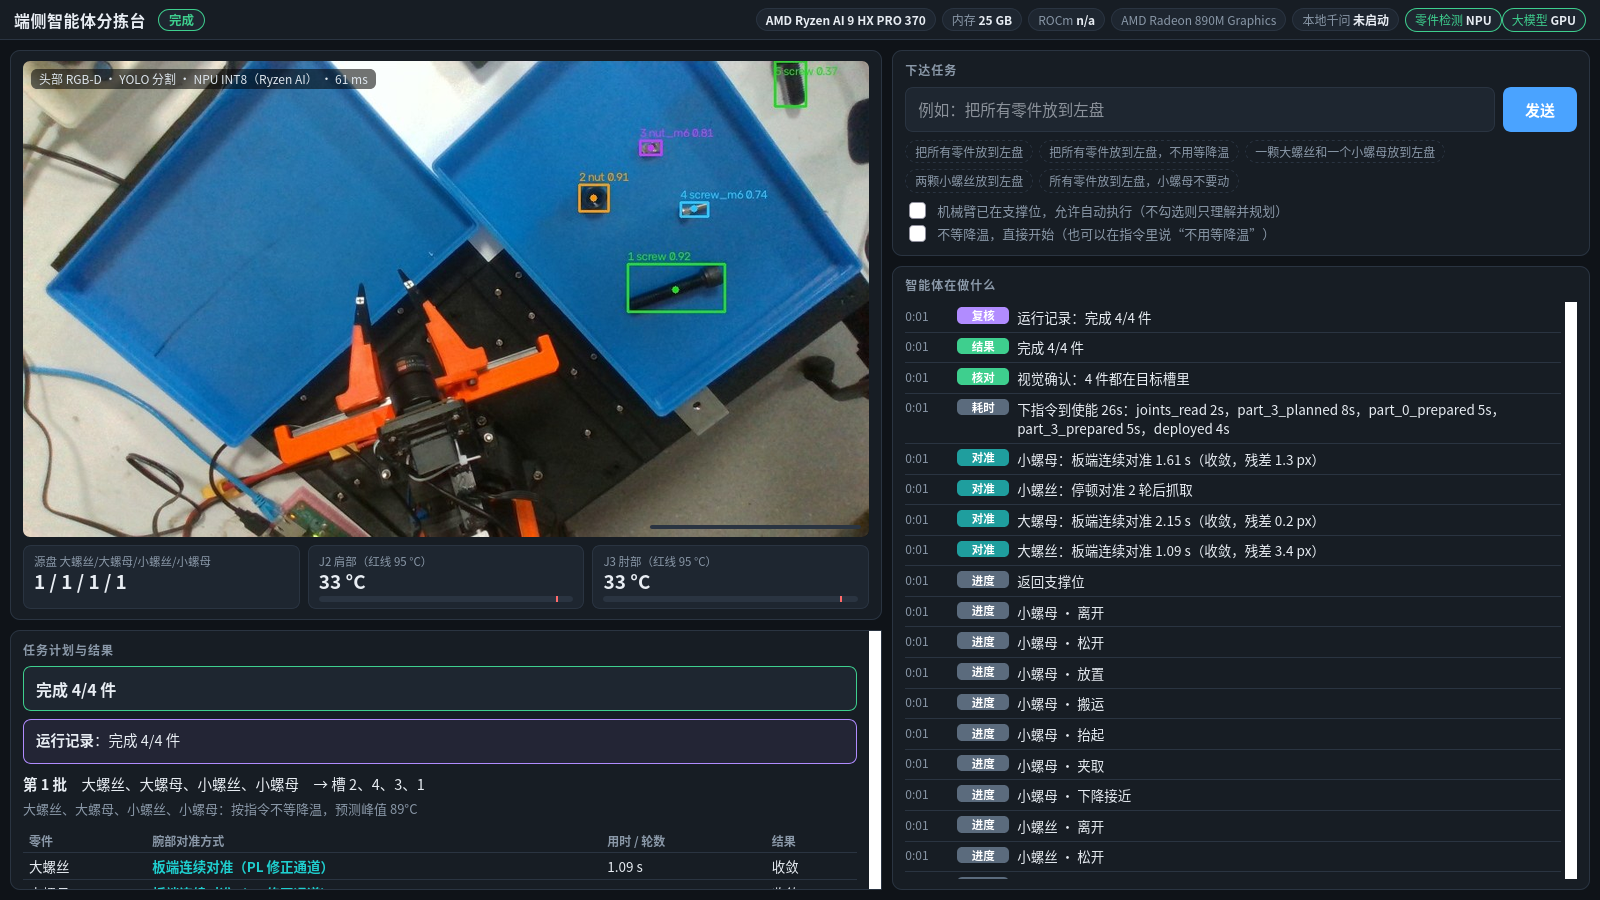
\includegraphics[width=.92\linewidth]{console_four_classes_npu.png}
  \caption{上位机控制台：指令、理解、执行进度、对准方式与复审一屏完成}\label{fig:console}
\end{figure}

\subsubsection{软件各模块介绍}

\begin{figure}[H]
\centering
\begin{tikzpicture}[
  font=\footnotesize,
  s/.style={draw=blue!60!black,fill=blue!6,rounded corners=2pt,align=center,minimum height=8mm,text width=26mm},
  d/.style={draw=orange!70!black,fill=orange!8,diamond,aspect=2.2,align=center,inner sep=1pt,text width=16mm},
  ar/.style={-{Stealth[length=1.6mm]},semithick},
  lab/.style={font=\scriptsize,fill=white,inner sep=1pt}]
  \node[s] (in) {中文指令};
  \node[d,below=4mm of in] (rule) {规则可解析？};
  \node[s,right=6mm of rule] (llm) {本地大模型\\生成候选合约};
  \node[s,below=4mm of rule] (val) {确定性校验\\→ 任务合约};
  \node[s,below=4mm of val] (per) {NPU 分割 + 深度\\→ 零件三维位姿};
  \node[s,below=4mm of per] (pl) {IK · 轨迹生成\\几何检查 · 作业包};
  \node[s,right=46mm of pl] (ex) {KV260 校验\\PL 5 ms 执行};
  \node[s,above=4mm of ex] (al) {腕部对准\\收敛 → 夹取};
  \node[s,above=4mm of al] (pp) {放置 · 返回起点};
  \node[s,above=4mm of pp] (rv) {头部相机核对\\大模型中文复审};
  \draw[ar] (in)--(rule); \draw[ar] (rule)--node[lab,left]{是}(val); \draw[ar] (rule)--node[lab]{否}(llm); \draw[ar] (llm)|-(val);
  \draw[ar] (val)--(per); \draw[ar] (per)--(pl); \draw[ar] (pl)--node[lab]{作业包}(ex);
  \draw[ar] (ex)--(al); \draw[ar] (al)--(pp); \draw[ar] (pp)--(rv);
\end{tikzpicture}
\caption{一次分拣任务的软件流程}\label{fig:swflow}
\end{figure}

\begin{table}[H]
\centering\small
\renewcommand{\arraystretch}{1.08}
\caption{软件模块与关键输入输出}\label{tab:sw}
\begin{tabularx}{\linewidth}{@{}p{2.3cm} Y Y Y@{}}
\toprule
模块 & 输入 & 处理 & 输出 \\
\midrule
指令理解 & 中文句子 & 规则或大模型解析；校验类别、数量和托盘 & 结构化任务 \path{workcell.task.v1} \\
零件感知 & RGB-D 帧 & 实例分割、深度定位、手眼坐标变换 & 基座坐标、主轴、置信度 \\
规划与校验 & 任务、零件位姿 & 逆运动学、轨迹生成、碰撞与速度检查 & 作业包与文件摘要 \\
板端执行 & 作业包 & 摘要校验、段提交、租约续期、事件回报 & PL 命令、执行事件 \\
腕部对准 & 腕部帧、目标点 & 图像定位；像素误差映射为关节偏移 & 修正目标、收敛信号 \\
核对与复审 & 前后画面、日志 & 逐槽计数；大模型对比前后画面 & 核验结果、中文说明 \\
示教与孪生 & 实测关节状态 & 重力补偿、拖动记录、三维渲染 & 关节姿态、轨迹记录 \\
\bottomrule
\end{tabularx}
\end{table}

\paragraph{两端协议。}AI PC 通过 SSH 传输作业包及板端运行文件，以内容摘要标识版本。停顿对准通过 HTTP 交换视觉请求和结果，使用唯一请求标识（nonce）、作业摘要和帧哈希关联当前任务。连续对准通过板内进程通信传递结果，修正计算无需往返 AI PC。

PS 通过 AXI-Lite 读写 PL 寄存器，图像核通过内存主接口读入灰度帧并写回掩码，PL 通过 CAN 29 位扩展帧发送电机设定。各入口分别检查文件一致性、数值范围和运行约束。PL 周期以硬件时钟计时，板端软件延迟以本机时钟计时，统计无需依赖跨机时钟同步。

\paragraph{腕部对准。}系统按零件类别处理腕部图像，提取抓取参考点，计算其与标定对准点之间的像素偏差。图像雅可比将偏差换算为工具平面位移，再映射为关节偏移写入 PL；PL 限制修正幅度和每周期变化量。图~\ref{fig:wrist} 展示图像处理各阶段。\doccite{ref:servo}

大螺丝、大螺母和小螺母采用板端连续对准，小螺丝采用停顿取图对准。大螺丝的手指区填充、高斯滤波、Otsu 阈值和闭运算由 PL 掩码核完成，后续轮廓定位由 PS 完成。连续对准按图像更新偏差，并以 100\,Hz 平滑写入修正目标；连续 3 帧满足阈值后进入下降和夹取。\doccite{ref:otsu}

\begin{figure}[H]
  \centering
  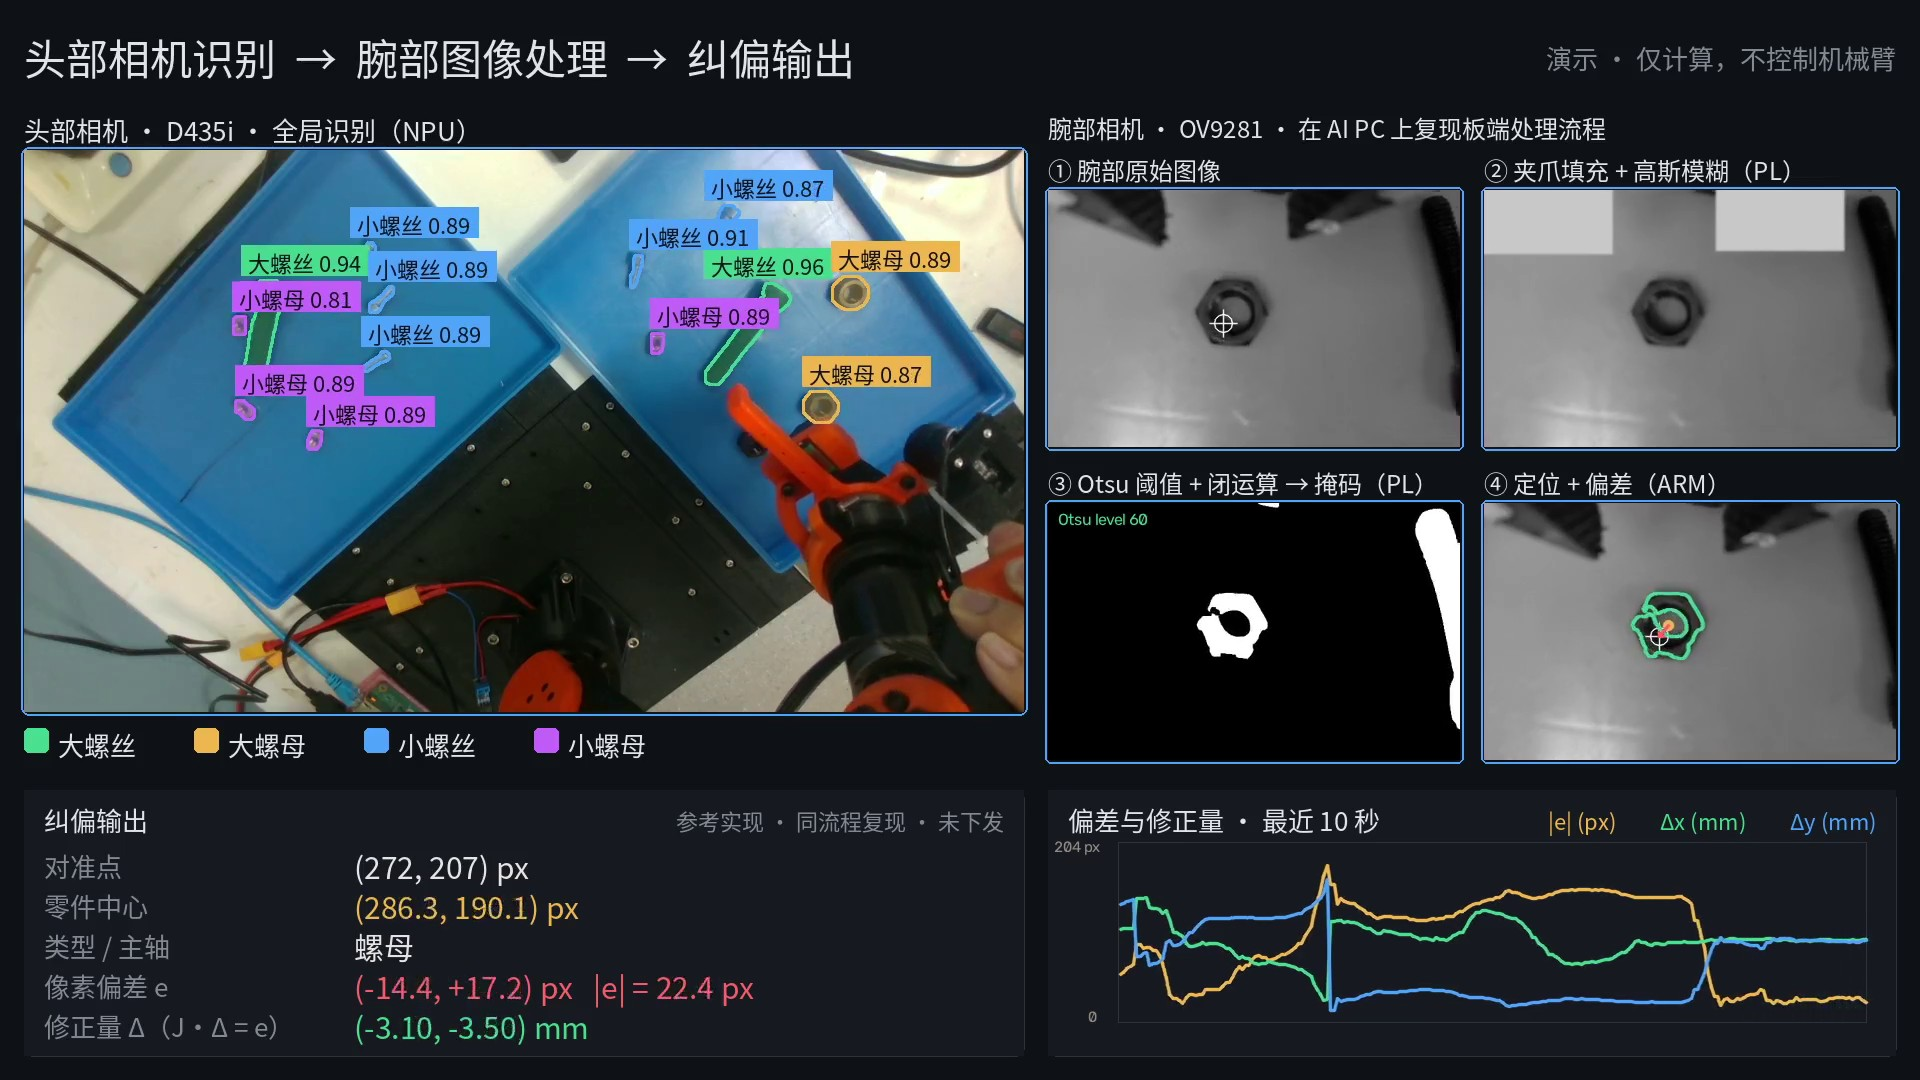
\includegraphics[width=\linewidth]{framework_view.jpg}
  \caption{头部识别与腕部图像处理流程（零重力手拖演示画面，腕部各阶段在 AI PC 上按板端流程复现）}\label{fig:wrist}
\end{figure}

\paragraph{零重力示教与数字孪生。}控制台启动零重力模式后，板端根据实测位姿计算重力补偿力矩，并施加三层力矩上限，辅助操作者手动拖动机械臂。控制台以 50\,ms 间隔读取关节角，通过 URDF 正运动学更新三维模型，并用测得速度补偿显示延迟。用户可记录指定点位的关节姿态或一段拖动轨迹，为点位配置与运动分析提供数据。